%%%%%%%%%%%%%%%%%%%%%%%%%%%%%%%%%%%%%%%%%%%%%%%%%%%%%%%%%%%%%%%%%%%%%%%%%%%%%%%%
%Objetivo: Introduzir os conceitos envolvidos na dissertação bem como do
%trabalho realizado. A ideia é que qualquer pessoa que leia a introdução
%consiga ter uma visão geral sobre a dissertação.
%Autor: Vagner Clementino<vagnercs@dcc.ufmg.br> e
%		Rodolfo Resende<rodolfo@dcc.ufmg.br>
%Criação: Dom Set 18 22:55:43 BRT 2016
%Modificação: qua set 13 21:46:54 -03 2017
%Revisão: ter jun  6 19:27:28 -03 2017
%%%%%%%%%%%%%%%%%%%%%%%%%%%%%%%%%%%%%%%%%%%%%%%%%%%%%%%%%%%%%%%%%%%%%%%%%%%%%%%%
\chapter{Introdução}\label{ch:intro}

Dentro do ciclo de vida de um produto de software o processo de Manutenção tem
papel fundamental. Devido ao seu alto custo, que pode variar entre 60\% e 90\%
do preço final do sistema~\cite{kaur2015review}, as atividades relacionadas com
manter e evoluir têm sua importância considerada tanto pela comunidade
científica quanto pela indústria. Uma vez que o software entra em operação,
anomalias são descobertas, mudanças ocorrem no ambiente de execução e o
atendimento a novos requisitos é solicitado. À frente caracterizamos o que
denominamos como ``Requisição de Mudança'' (RM) e o nosso interesse em um tipo
de ferramenta que denominamos \texttt{``Ferramentas de Gerenciamento de
    Requisições de Mudanças'' (FGRM)}. De uma maneira informal uma RM
representa uma solicitação de manutenção e a FGRM dá apoio às atividades de
gerência destas solicitações. Esta dissertação apresenta o estudo de FGRMs
feito no correspondente projeto de mestrado e apresenta contribuições sobre
como melhorar este tipo de software.

A \textit{Manutenção}, dentre outros aspectos, corresponde ao processo de
modificar um componente ou sistema de software após a sua entrega com o
objetivo de \textit{corrigir falhas, melhorar o desempenho ou adaptá-lo devido
    à mudanças ambientais}~\cite{{159342}}. De maneira relacionada,
\textit{Manutenibilidade} é a propriedade de um sistema ou componente de
software em relação ao grau de \textit{facilidade} que ele pode ser corrigido,
melhorado ou adaptado~\cite{{159342}}. As manutenções de software, conforme
apresenta a Figura~\ref{fig:modification-request} podem ser divididas em
\textit{Corretiva, Adaptativa, Perfectiva e
    Preventiva}~\cite{Lientz:1980:SMM:601062,159342}. A Manutenção Corretiva
lida com a reparação de falhas encontradas. A Adaptativa tem o seu foco na
adequação do software por conta de mudanças ocorridas no ambiente em que ele
está inserido. A Perfectiva trabalha para detectar e corrigir falhas latentes
antes que elas se manifestem como tal. A Preventiva se preocupa com atividades
que possibilitem aumento da manutenibilidade do sistema. A ISO 14764 propõe que
exista um elemento denominado Requisição de Mudança (RM) que corresponde a uma
agregação de características que representam uma solicitação de manutenção de
qualquer das quatro categorias. Nesta dissertação adotamos a mesma terminologia
com o mesmo significado.

\begin{figure}[hbtp] \centering 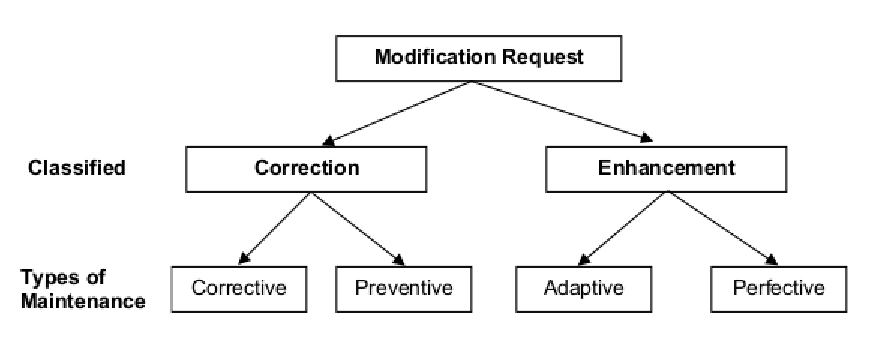
\includegraphics[width=.75\textwidth]
	{./chapter-intro/img/modification_request.eps} \caption{Tipos de manutenção
		segundo a norma ISO/IEC 14764. Extraído de~\cite{1703974}}
\label{fig:modification-request} \end{figure}

Por conta do volume das RMs, é importante a utilização de um software para
gerenciá-las. Esse controle é realizado pelas FGRMs que auxiliam a equipe de
manutenção na correção, de forma individual ou colaborativa, de falhas (bugs)
ou na implementação de melhorias. Estas ferramentas podem ser utilizadas por
gestores, analistas de qualidade e usuários do sistema para atividades como
gerenciamento de projetos, comunicação, discussão e revisões de código. A
literatura sobre Manutenção de Software não define uma nomenclatura comum para
este tipo de software. Em alguns estudos são utilizados nomes como Sistema de
Rastreio de Defeito~-~\textit{Bug Tracking Systems}, Sistema de Gerenciamento
de Requisição~-~\textit{Request Management System}, sendo bastante comum o
termo Sistemas de Controle de Demandas~-~\textit{Issue Tracking Systems}.
Todavia, de modo geral, o termo se refere às ferramentas utilizadas no
\textit{gerenciamento das Requisições de Mudança}. Nesta dissertação utilizamos
o termo Ferramentas de Gerenciamento de Requisições de Mudança (FGRM) ao
referirmos a este tipo de software. A Tabela~\ref{tab:exemplo} apresenta alguns
exemplos de sistemas que podem ser classificados como FGRMs. Também são
listados serviços da Internet que oferecem funcionalidades existentes nas FGRMs
na modalidade de Software como Serviço~\cite{fox2013engineering}.

\begin{table}[htpb]
\centering
\resizebox{\textwidth}{!}{%
\begin{tabular}{@{}clll@{}}
\toprule
\multicolumn{2}{c}{Ferramentas}                   & \multicolumn{2}{c}{Serviços da Internet} \\ \midrule
Bugzilla & https://www.bugzilla.org/               & SourceForge  & https://sourceforge.net/  \\ \midrule
MantisBT & https://www.mantisbt.org/               & Lauchpad     & https://launchpad.net/    \\ \midrule
Trac     & https://trac.edgewall.org/              & Code Plex    & https://www.codeplex.com/ \\ \midrule
Redmine  & www.redmine.org/                        & Google Code  & https://code.google.com/  \\ \midrule
Jira     & https://www.atlassian.com/software/jira & GitHub       & https://github.com/       \\ \bottomrule
\end{tabular}%
}
\caption{Exemplos de ferramentas e serviços da Internet que podem ser
    classificados como FGRMs. Extraído de~\cite{cavalcanti2014challenges}}
\label{tab:exemplo}
\end{table}

\section{Motivação}
\label{sec:intro-motivacao}

Diante da maior presença de software em todos os setores da sociedade existe um
interesse por parte da comunidade científica e da industria no desenvolvimento
de processos, técnicas e \textit{ferramentas} que melhorem a relação
custo/benefício de manter um software. Dependendo do tamanho do projeto de
software é necessário a utilização de uma FGRM para gerenciar as suas
requisições de mudança. Além disso, as diferentes partes interessadas
necessitam de um espaço único onde possam registrar as falhas encontradas e as
melhorias que necessitam. Neste contexto, verificamos que as FGRMs fazem parte
de projetos de diferentes tipos e tamanhos, em empresas públicas e privadas
(por exemplo NASA e IBM) e de diversos projeto de código aberto (por exemplo
Mozilla, Eclipse, Apache); elas dão suporte a softwares de diferentes
plataformas: computadores de mesa, web ou dispositivos móveis.

A literatura mostra que uma FGRM desempenha um papel além do gerenciamento dos
pedidos de manutenção de software. Avaliando o controle de demandas como um
processo social, Bertram e outros~\cite{Bertram:2010:CCB:1718918.1718972}
realizaram um estudo qualitativo sobre FGRMs que eram utilizadas por equipes de
pequeno porte. Os resultados demonstraram que a ferramenta era utilizada não
apenas como um banco de dados de rastreamento de falhas, mas atuava como um
ponto central para a comunicação e coordenação das diversas partes interessadas
dentro e fora da equipe de manutenção. Os clientes, gerentes de projeto,
analistas de qualidade e programadores contribuíam em conjunto para o
compartilhamento do conhecimento do projeto através da FGRM utilizada.

No trabalho de Breu e outros~\cite{breu2010information} o foco foi
analisar o papel das FGRMs no suporte à colaboração entre desenvolvedores e
usuários de um software. Com base nos resultados foi possível verificar que o
uso da ferramenta possibilitou que os usuários desempenhassem um papel além de
simplesmente reportar uma falha: a participação ativa e permanente foi
importante no progresso da solução das falhas que eles descreveram. Um outro
benefício das FGRMs é que as mudanças no software podem ser rapidamente
identificadas e reportadas para os desenvolvedores~\cite{anvik2005coping}. Além
disso, elas podem ajudar na estimativa do custo do software, na análise do
impacto de uma modificação, no planejamento do projeto, na rastreabilidade de
uma falha e na extração de conhecimento~\cite{cavalcanti2013bug}.

Conforme exposto, as FGRMs desempenham um papel fundamental no contexto do
desenvolvimento e manutenção de software. Entretanto, no escopo de sua
utilização diversos desafios se apresentam: duplicação de RMs, pedidos de
modificação abertos inadvertidamente, grande volume de RMs que devem ser
atribuídas aos desenvolvedores, RMs descritas de forma
incompleta~\cite{cavalcanti2014challenges}. Diante destes problemas e desafios
é importante entender como estas ferramentas estão sendo utilizadas e o que
está sendo proposto na literatura sobre elas, de modo a avaliar e entender as
necessidades dos profissionais envolvidos com Manutenção de Software visando
propor melhorias paras as funcionalidades oferecidas pelas FGRMs.

\section{Problema}
\label{sec:intro-problema}

O desenvolvimento e a manutenção de software envolvem diversos tipos de métodos,
técnicas e ferramentas. Em especial no processo de Manutenção, um importante
aspecto são as diversas RMs que devem ser gerenciadas, cujo controle é realizado
pelas FGRMs. Apesar da inegável importância dessa ferramenta, percebe-se um
aparente desacoplamento de suas funcionalidades com as necessidades das diversas
partes interessadas na manutenção e evolução de software. A utilização de
\textit{``demanda''} como conceito central para as FGRMs parece ser distante das
necessidades práticas dos projetos de software, especialmente no ponto de vista
dos desenvolvedores~\cite{Baysal:2013:SAP:2486788.2486957}.

Um exemplo deste desacoplamento pode ser visto no trabalho proposto por Baysal
e Holme~\cite{baysal2012qualitative} no qual desenvolvedores que utilizam o
Bugzilla\footnote{\url{https://www.bugzilla.org}} relataram dificuldade em
manter uma compreensão do escopo que as RMs atribuídas para eles possuem.
Segundo eles, seria importante que a ferramenta tivesse um suporte melhorado
para o conceito de Percepção Situacional~-~Situational Awareness. Em síntese,
eles gostariam de estar cientes da situação global do projeto bem como das
atividades que estavam sendo desempenhadas pelo demais desenvolvedores.

Existem outros problemas que são potencializados pela ausência de certas
funcionalidades nas FGRMs. Uma amostra são as ferramentas que permitem a
inclusão de RMs com relatos de baixa qualidade. Nesta situação os usuários
terminam por serem solicitados a inserir mais informação sobre as quais algumas
das vezes não têm conhecimento. Por outro lado, verifica-se uma frustração por
parte dos desenvolvedores que não conseguem realizar o seu trabalho por conta
da ausência da informação que necessitam~\cite{just2008towards}.

Corroborando com a necessidade de evolução das FGRMs, o estudo realizado por
Zimmermann e outros~\cite{zimmermann2009improving} propõe quatro dimensões de
melhorias para este tipo de software. Estas dimensões representam
aperfeiçoamentos centrados em aspectos tais como \textit{ferramenta, informação,
    processo e usuário}. Eles são melhor discutidos no
Capítulo~\ref{ch:mapeamento-sistematico} onde foram utilizados na classificação
de estudos no Mapeamento Sistemático realizado.

Não encontramos um grande número de trabalhos que avaliam de forma sistemática
as funcionalidades oferecidas pelas FGRMs, ao mesmo tempo que faça relação com
que vem sendo proposto na li\-te\-ra\-tu\-ra sobre o assunto.  Adicionalmente,
os estudos sobre melhorias das FGRMs não discutem a adoção de algumas das
práticas propostas pelos agilistas na Manutenção de Software~\cite{Soltan2016,
    Heeager2015}. É importante que as FGRMs evoluam para se adaptar a esta
forma de trabalho. Um outro fator que corrobora sobre a necessidade de
melhorias das FGRMs são as diversas extensões (\textit{plugins}) propostas na
literatura
\cite{101186,Thung:2014:BIT:2635868.2661678,Kononenko:2014:DED:2591062.2591075}.

\section{Objetivos}
\label{sec:intro-objetivos}

Segundo o nosso entendimento existe um distanciamento entre as necessidades dos
profissionais envolvidos em Manutenção de Software e as funcionalidades
oferecidas pelas FGRMs\@. Por esta razão, este trabalho de dissertação investiga
e contribui no entendimento de como as FGRMs podem ser melhoradas ou estendidas
no contexto da transformação do processo de desenvolvimento e manutenção de
software de um modelo tradicional para outro que incorpora cada vez mais as
práticas propostas pelos agilistas. O intuito é analisar como as FGRMs estão
sendo modificadas com base na literatura da área em contraste com o ponto de
vista dos profissionais envolvidos com manutenção. Neste sentido, elaboramos um
estudo sobre as FGRMs com os seguintes objetivos:

\begin{enumerate}[(i)]
	\item entender os requisitos e funcionalidades oferecidas por este tipo de
        ferramenta;
	\item mapear as melhorias para as FGRMs que estão sendo propostas na
		literatura;
    \item verificar como os profissionais avaliam as funcionalidades das
        ferramentas que têm contato;
	\item propor melhorias para as funcionalidades das FGRMs\@.
\end{enumerate}

%Vamos discutir os aspectos que são considerados mais importantes a partir da
%literatura da área, bem como do ponto de vista de profissionais envolvidos em
%manutenção de software. De forma particular, iremos estudar os mecanismos de
%personalização que algumas destas ferramentas permitem e tentaremos ainda criar
%exemplos de personalização para alguma possível extensão a ser identificada ao
%longo do trabalho.

\section{Visão Geral da Dissertação}
\label{sec:intro-visao-geral}

A fim de alcançarmos os objetivos descritos foi proposto um conjunto de
melhorias para as funcionalidades das FGRMs. As sugestões de aperfeiçoamento
são apresentadas no Capítulo~\ref{ch:sug_melhoria} e foram baseadas no
\textit{(i)} mapeamento apresentado no Capítulo~\ref{ch:mapeamento-sistematico}
e no \textit(ii) levantamento com profissionais descrito no
Capítulo~\ref{ch:pesquisa-profissionais}. O Capítulo~\ref{ch:sug_melhoria} além
de sugerir melhorias realizou um levantamento (\textit{survey}) da percepção
destas recomendações por parte de profissionais de desenvolvimento de software.

Mediante o mapeamento sistemático obtivemos e avaliamos uma parte das melhorias
para as funcionalidades das FGRMs que estavam sendo propostas na literatura. A
partir do estudo foi possível propor dois esquemas de classificação: por
dimensão de melhoria e suporte ao papel desempenhado na manutenção de software.
De maneira similar, através da caracterização das funcionalidades de algumas
FGRMs de código aberto ou disponíveis comercialmente, identificamos o estado da
prática deste tipo de ferramenta.

Com base nestes dois estudos conduzimos uma pesquisa com profissionais em que
pedimos que avaliassem os requisitos funcionais e não funcionais que poderiam
ser utilizados para aperfeiçoar as FGRMs. O questionário também quis saber a
opinião dos profissionais sobre a relevância das propostas de me\-lho\-ri\-as
existente na literatura em sua rotina de trabalho. Fundamentado nos estudos
descritos foi proposto um conjunto de melhorias. Como prova de conceito e em
função de restrições de tempo escolhemos implementar apenas uma delas conforme
descrito no Capítulo~\ref{ch:implemtacao_extensao}.

\section{Metodologia de Pesquisa}
\label{sec:intro-metodologia}

A metodologia de pesquisa utilizada neste estudo é baseada em uma abordagem
multi-método~\cite{hesse2010mixed}. Este tipo de desenho combina dois ou mais
métodos quantitativos ou qualitativos em um único estudo. As etapas do
trabalho, que compõem a abordagem multi-método estão listadas a seguir:

\begin{enumerate}[(i)]
	\item Mapeamento Sistemático da Literatura~\cite{Petersen2008}
	\item Caracterização das funcionalidades das FGRMs
    \item Levantamento (\textit{Survey}) com
          desenvolvedores~\cite{wohlin2012experimentation}
	\item Proposição e avaliação de um conjunto de melhorias para as FGRMs
    \item Implementação, como Prova de Conceito, de uma extensão para
        determinada FGRM
\end{enumerate}

\section{Contribuições do Estudo}
\label{sec:intro-contribuicao}

Este estudo sistematizou uma parte da literatura sobre melhorias das
funcionalidades das FGRMs ao mesmo tempo que avaliou com base na opinião de
profissionais envolvidos com desenvolvimento e manutenção de software a
relevância de tais alterações. Além disso, foi proposto um conjunto de
recomendações que podem contribuir com a melhoria das funcionalidades
disponibilizadas por este tipo de software. Uma das recomendações foi
implementada demonstrando a aplicabilidade do que foi apresentado. Entendemos
que uma FGRM que atenda as necessidades dos desenvolvedores possa contribuir
com o aperfeiçoamento das atividades relacionadas com manutenção de software e
na diminuição de custos. Neste sentido, entendemos que contribuímos no avanço
dos estudos sobre melhorias das FGRMs. Os resultados apresentados nesta
dissertação podem ser utilizados para o desenvolvimento de novas versões para
este tipo de software ou serem aplicados pela equipe de manutenção para
otimizar a sua rotina de trabalho.

\section{Organização do Trabalho}
\label{sec:intro-organizacao-dissertacao}

Este trabalho de dissertação está organizado conforme descrito a seguir. No
Capítulo~\ref{ch:visao-geral-manutencao} apresentamos e discutimos os principais
conceitos utilizados nesta dissertação. Neste mesmo capítulo é descrito um
estudo em que coletamos as funcionalidades de um conjunto de FGRMs que foram
definidas como relevantes na visão de profissionais consultados mediante um
levantamento.

O Capítulo~\ref{ch:mapeamento-sistematico} descreve o mapeamento sistemático que
trata de trabalhos sobre melhorias nas funcionalidades das FGRMs. Os estudos
foram classificados em 04 dimensões de melhorias e pelo papel desempenhado na
Manutenção de Software que a melhoria visa dar suporte. No
Capítulo~\ref{ch:pesquisa-profissionais} reunimos a opinião de profissionais
envolvidos em Manutenção de Software sobre as funcionalidades oferecidas pelas
FGRMs. Estes profissionais exercem suas atividades em projetos de código aberto
e empresas do setor público e privado. Foi possível identificar que os
participantes do levantamento, na maior parte, estão satisfeitos com a
ferramenta que utiliza, contudo, eles se mostram interessados em novos tipos de
funções para este tipo de software.

Tomando como base a literatura sobre melhorias nas FGRMs e os resultados obtidos
nos estudos descritos em capítulos anteriores, apresentamos e discutimos um
conjunto de recomendações para as funcionalidades das FGRMs no
Capítulo~\ref{ch:sug_melhoria}. As sugestões propostas foram avaliadas por
profissionais que contribuem no desenvolvimento deste tipo de ferramenta. Em
geral, as recomendações tiveram boa aceitação com relação à sua necessidade e
facilidade de implementação. O Capítulo~\ref{ch:implemtacao_extensao} descreve a
implementação de uma das 8 sugestões propostas. O
Capítulo~\ref{ch:conclusao_trab_futuros} apresenta uma discussão final e também
apresenta algumas recomendações de trabalhos futuros.
